% Draft of the body subsection on the kinetic loss (fork L1, 1 Oct 2026).  To be placed in the theory section, after the
% saturation of the instability; the figure belongs with the comparison against the simulations.  No simulation numbers.
% ---- BLOCK 1 (theory): replaces the body's subsection 'The kinetic loss' (label sec:loss) and its equation (label eq:loss)
\subsection{The kinetic loss}\label{sec:loss}

A flute-like vortex in the fluid limit conserves its energy. The vortices are damped because they are not quite flute-like. The field equation \cref{eq:poisson} contains \(\nabla_\perp^2\), whose two parts, radial and binormal, vary differently along the field line, so a potential that is constant along the line cannot satisfy it at every point: the charge of a fluid element, as it is carried round the vortex, changes by slightly different amounts at different points of the same field line. The difference is made up by currents along the line, and these require a parallel electric field, i.e., a small part \(\varphi_1\) of the vortex potential that varies along the line. We show in \cref{app:landau} that
\begin{equation}
\varphi_1 = k^2\lambdaD^2\,\chi(l;\wt)\,\varphi_0,
\label{eq:nonflute}
\end{equation}
where \(\varphi_0\) is the flute-like part, \(\wt = \omega - kU\) is the frequency of the vortex as seen by the plasma that the zonal flow carries past it, and \(\chi\) is a function along the field line that the magnetic geometry fixes, through \cref{eq:Hchi}. The non-flute part is therefore small, of relative size \(k^2\lambdaD^2\), and proportional to the amplitude of the vortex.

A parallel electric field that oscillates at the frequency \(\wt\) does work on the particles whose motion along the field line keeps step with it, viz., those whose transit or bounce frequency \(\omega_\tau\) satisfies \(n\omega_\tau = \wt\) for some integer \(n\). This is Landau damping \citep{Landau1946}. It converts the electrostatic energy of the vortex into fine structure of the distribution in the parallel velocity, i.e., into entropy, which the sinks then remove; the rate of conversion does not depend on the sinks. Since \(\wt\) is comparable with the transit frequency of a thermal particle over most of the width of a vortex, the resonant particles are thermal ones, and the damping of \(\varphi_1\) is strong; the damping of the vortex is weak only because \(\varphi_1\) is small. The result of \cref{app:landau} is
\begin{equation}
\frac{L}{\Enz} = 2\,k^2\lambdaD^2\,
\frac{\displaystyle k^2\int\rmd x\,|\varphi_0|^2\,\Dfn\!\left(\omega - kU\right)}
{\displaystyle\int\rmd x\left(\langle g^{xx}\rangle|\partial_x\varphi_0|^2 + \langle g^{yy}\rangle k^2|\varphi_0|^2\right)},
\label{eq:loss}
\end{equation}
where \(L\) is the rate at which the vortices lose electrostatic energy, the angle brackets denote the average along the field line, and the dissipation function \(\Dfn(\wt) = -\wt\langle s\operatorname{Im}\chi\rangle\), with \(s(l)\) the geometrical factor \cref{eq:Hsource}, measures the part of \(\varphi_1\) that lags behind its forcing. It vanishes for \(\wt\) small compared with the transit frequency, which is the limit of the transit-averaged equations of \cref{sec:equations}, and peaks where \(\wt\) is a few times the transit frequency.

Equation \cref{eq:loss} has no adjustable parameter, and it makes three statements that can be tested. Firstly, the loss rate is independent of the amplitude of the vortices: the damping is linear, whatever the state of the trapped fluid in their cat's eyes. Secondly, it is of the order of \(k^2\lambdaD^2\) times the transit frequency, so the vortices of a larger box are damped more slowly. Thirdly, the lag of the non-flute potential, measured at any radius, on either vortex and at any time, is a single function of the local value of \(\wt\).

% ---- BLOCK 2 (comparison with the simulations): paragraph and figure for the subsection on the energy budget (label sec:dissipation)
All three statements of \cref{sec:loss} about the kinetic loss hold (see \cref{fig:landau}). The measured lag falls on the predicted \(\Dfn(\wt)\) wherever the vortices are appreciable. The loss rate measured by the energy diagnostics of the code, in the channel of parallel streaming, is the predicted one throughout the decay of the reduced-box run, while the energy of the vortices falls by orders of magnitude; it is the same in the restarts with reduced amplitude; and in the production run of \citet{KennedyPlunkLetter}, whose box is four times larger in each perpendicular direction, it is smaller by the predicted factor.

\begin{figure}
\centering
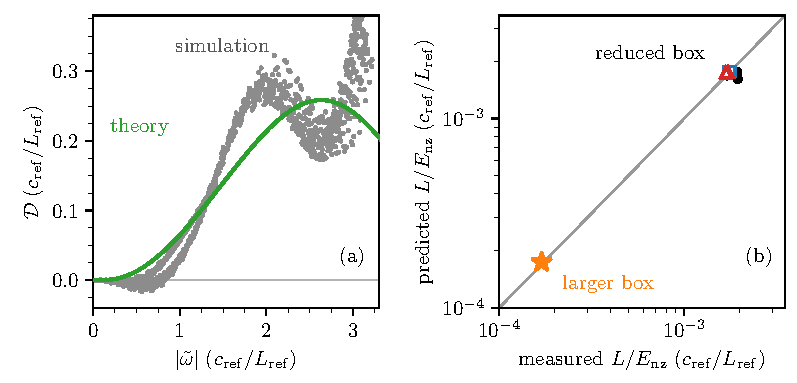
\includegraphics{figures/landau.pdf}
\caption{Landau damping of the non-flute part of the vortices: theory against simulation. (a) The dissipation function \(\Dfn\) of \cref{eq:Hdissipation} against the local Doppler-shifted frequency \(|\wt|\): the solution of \cref{eq:Hchi} in the magnetic geometry of the flux tube (green line), and its measured counterpart, viz., the part of the non-flute potential that lags behind its forcing, at every radius where either vortex is appreciable and at many times through the decay of the reduced-box run (grey dots). (b) The loss rate \(L/\Enz\) predicted by \cref{eq:loss} from the flute-like part of the vortices and the jets, against the rate measured by the energy diagnostics of the code in the channel of parallel streaming, for the reduced-box run through its decay (black dots), its \(\epsilon = 0.3\) (blue squares) and \(\epsilon = 0.03\) (red triangles) restarts, and the production run of \citet{KennedyPlunkLetter}, whose box is four times larger in each perpendicular direction (orange star); the line is equality. The vortices lose their energy by Landau damping of their non-flute part, at the rate that the theory gives, with no adjustable parameter, in every run.}
\label{fig:landau}
\end{figure}
